\chapter{Конструкторский раздел}

В данном разделе представлены схемы алгоритмов DBSCAN и его модификации.

\section{Разработка алгоритмов}
 
На рисунке \ref{fig:alg} приведена схема плотностного алгоритма DBSCAN.

\begin{figure}[ht!]
	\centering
	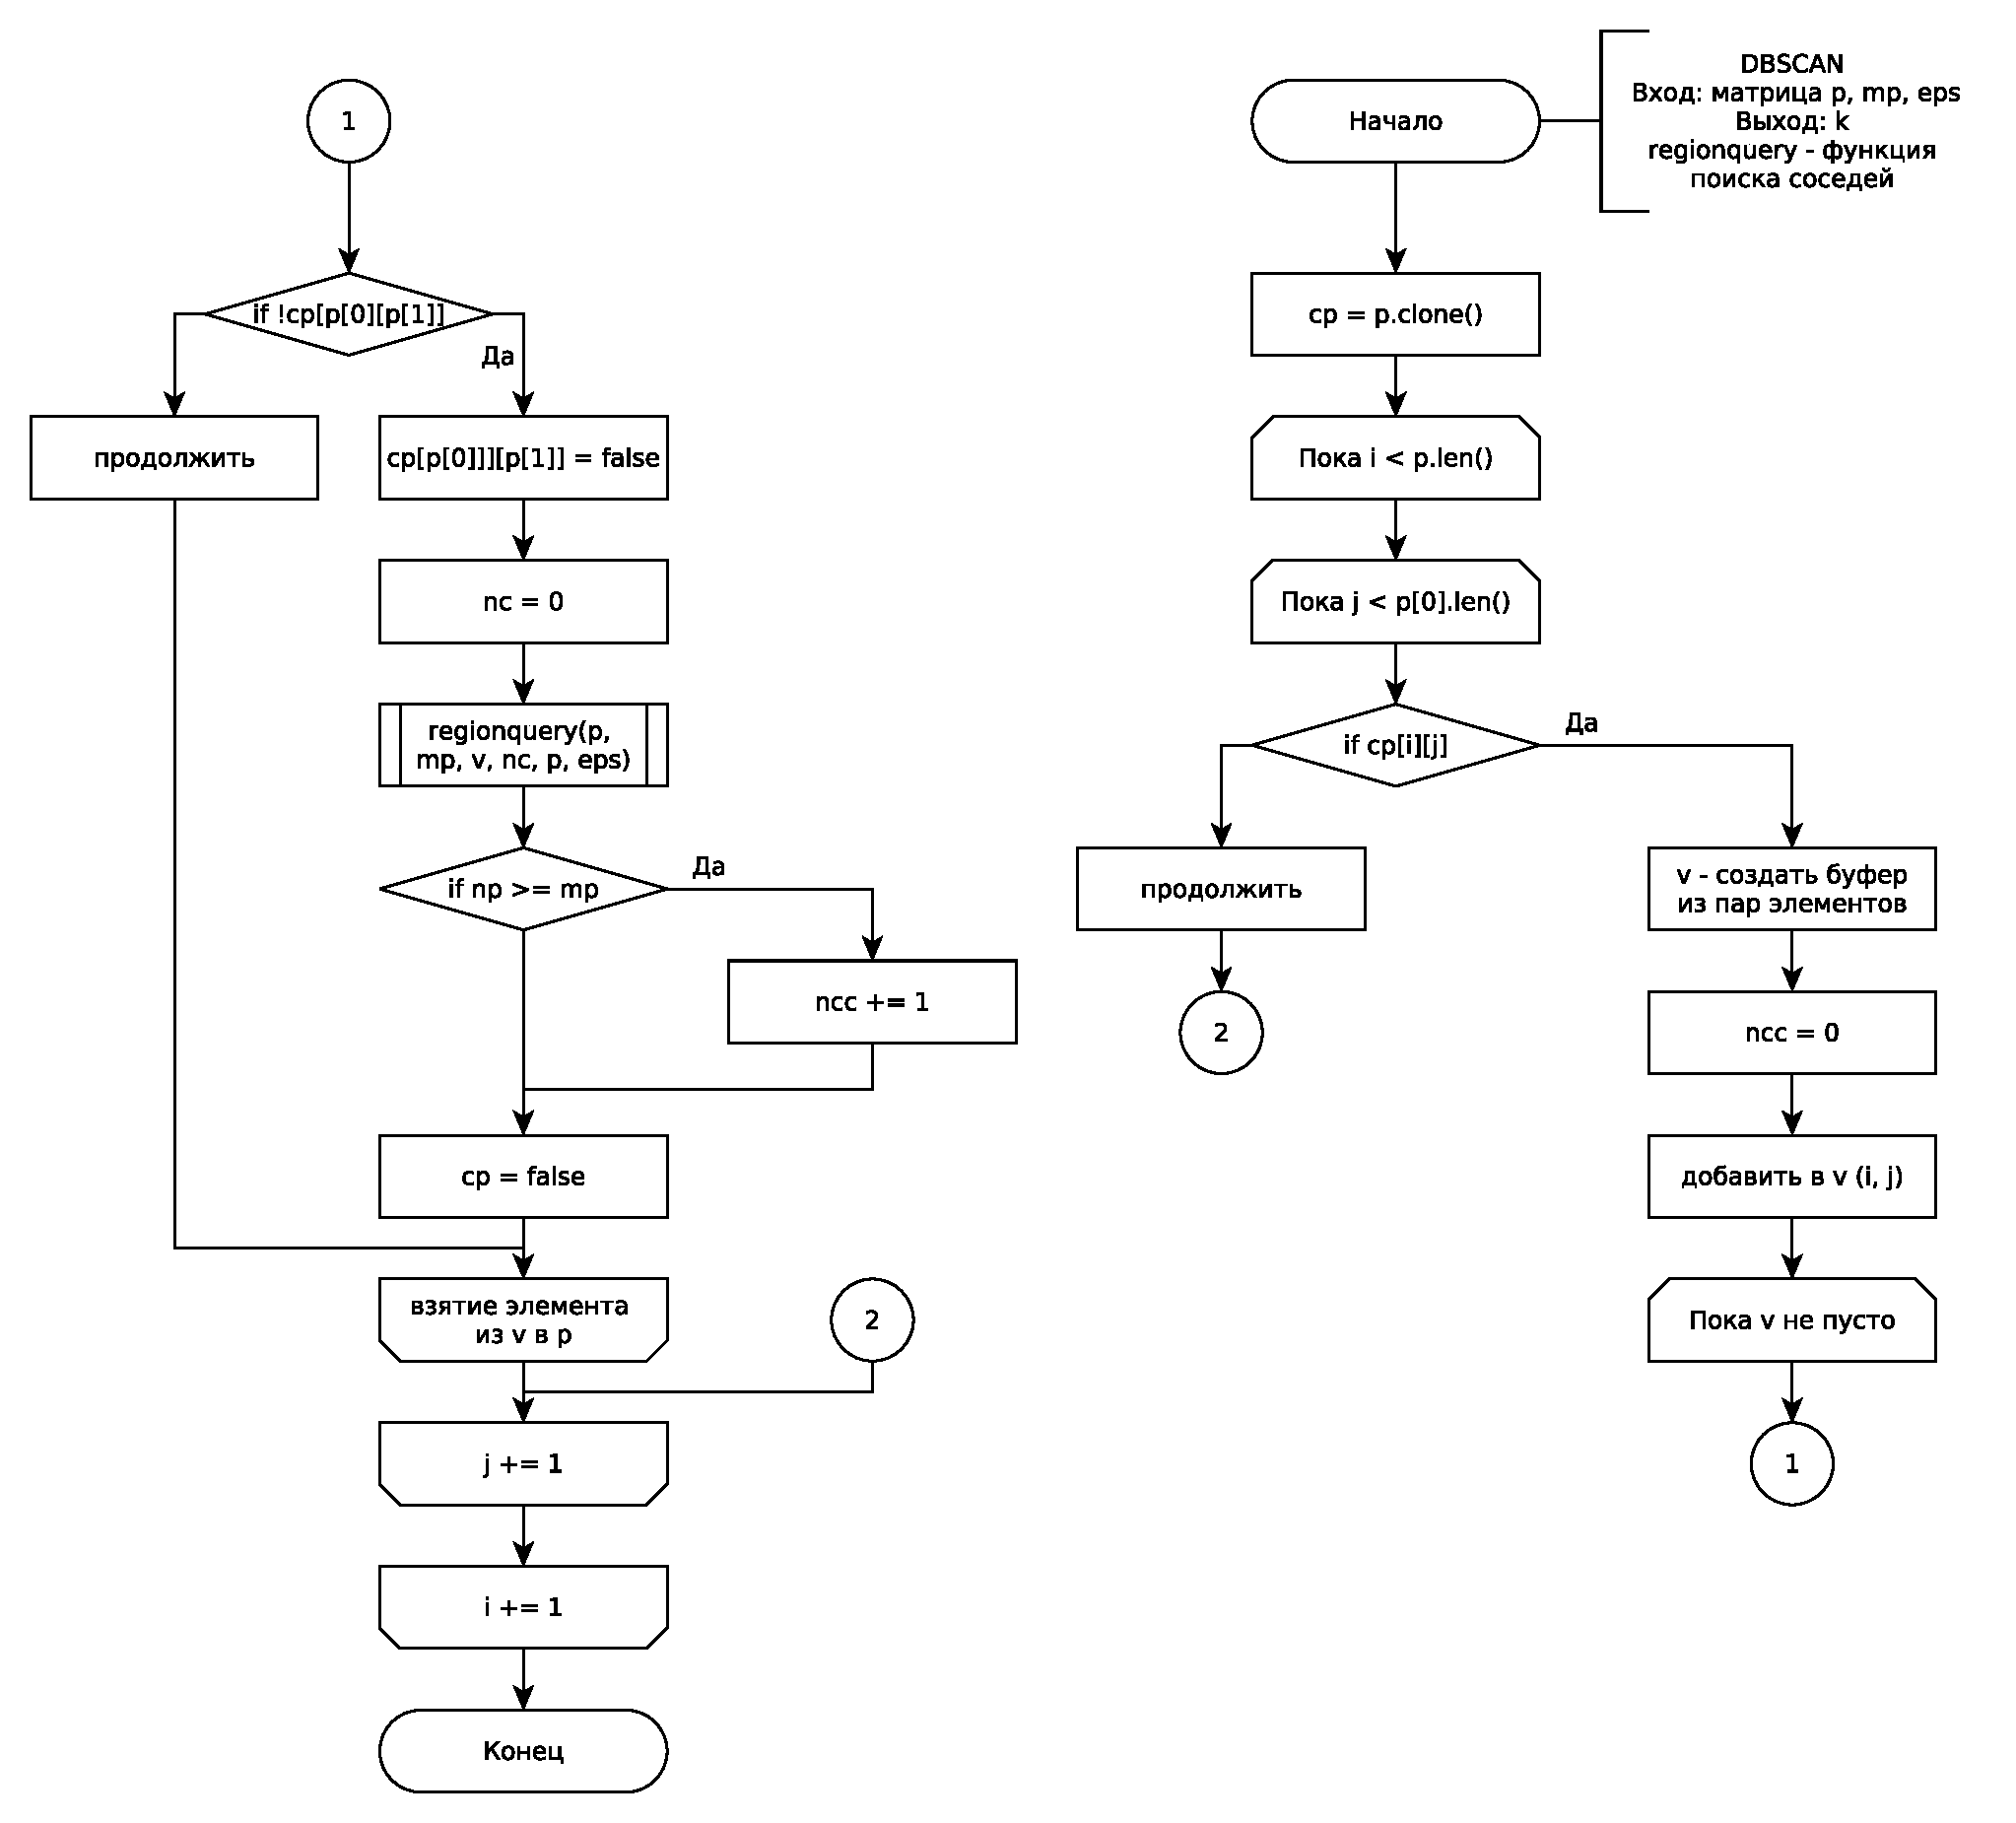
\includegraphics[width=1\linewidth]{assets/graphs/dbscan.pdf}
	\caption{Схема плотностного алгоритма DBSCAN}
	\label{fig:alg}
\end{figure}

На рисунке \ref{fig:alg2} приведена схема функции поиска ближайшей соседний точки в кластере.

\begin{figure}[ht!]
	\centering
	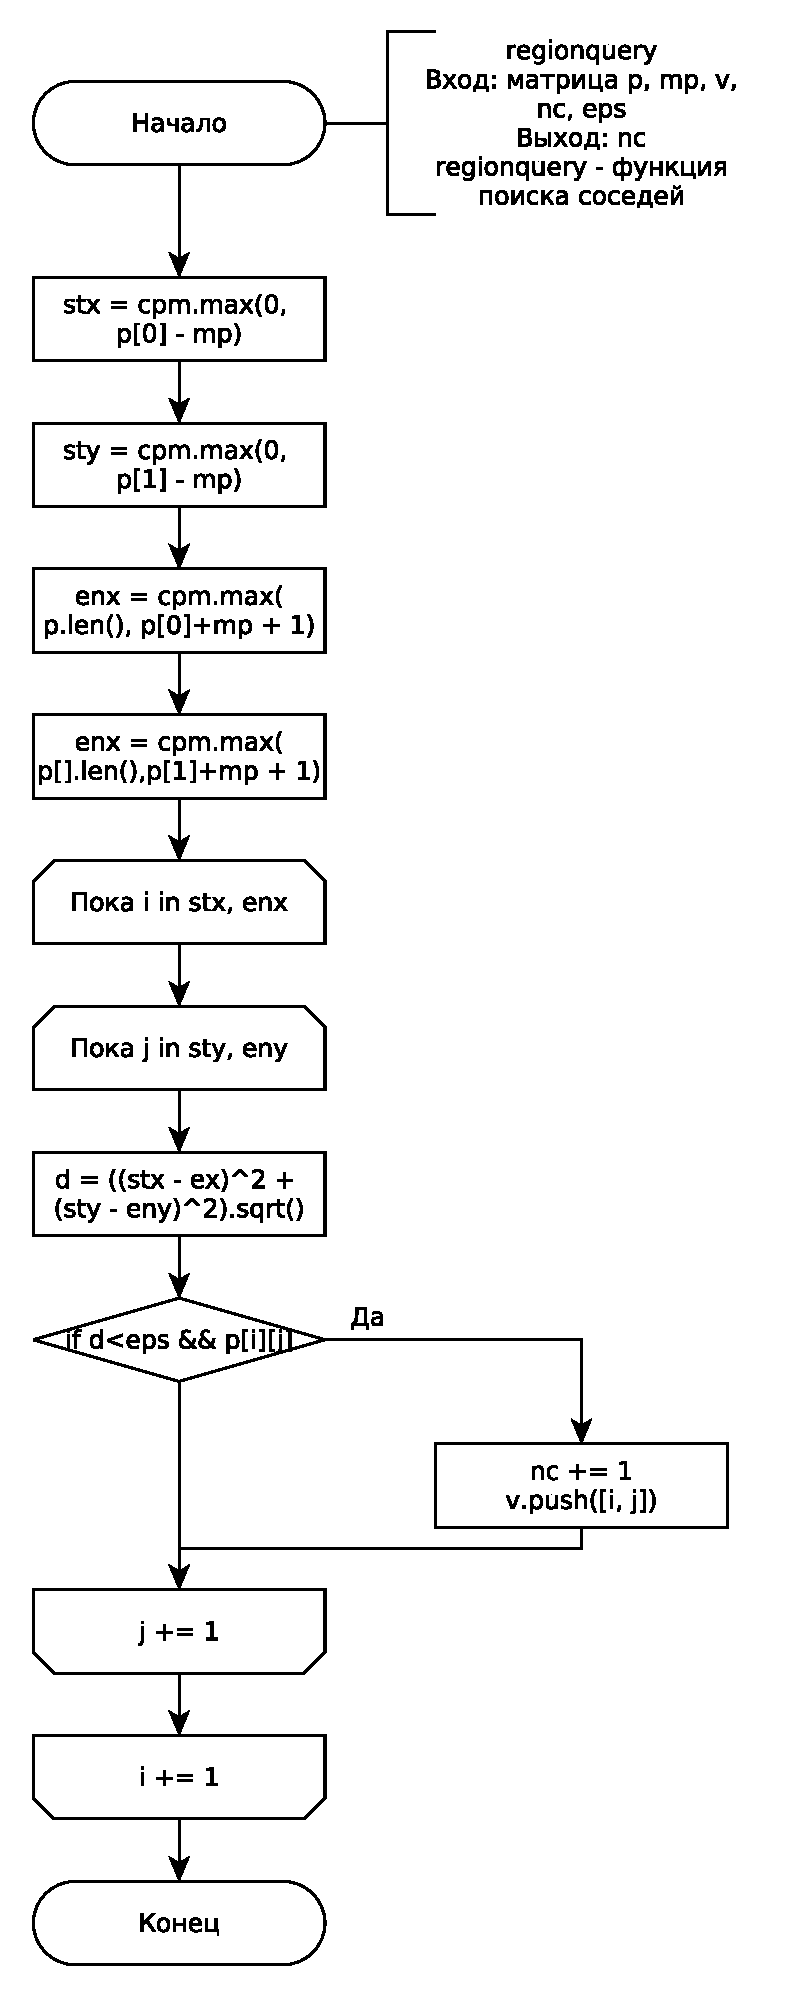
\includegraphics[width=0.5\linewidth]{assets/graphs/regionquery.pdf}
	\caption{Схема функции regionquery}
	\label{fig:alg2}
\end{figure}

\subsection{Параллельная реализация алгоритма DBSCAN}


Пусть размеры входной матрицы равны $M \times K$.

Рассмотрим необходимые для распараллеливания замечания:
\begin{itemize}
	\item каждый из выделенных этапов может быть выполнен независимо от других;
	\item в следствие независимости этапов, каждый их них может быть выполнен в любой момент, в том числе и параллельно с другими;
	\item каждый из выделенных этапов содержит цикл в некотором промежутке, который может быть разбит на некоторое множество меньших промежутков, в сумме составляющих исходный;
	\item трудоёмкости первого и второго этапов - величины одного порядка и относятся $M / N$;
	\item трудоёмкость третьего этапа в $N$ раз больше трудоёмкости первого этапа и в $M$ раз больше трудоёмкости второго этапа, что, не позволяет распараллелить третий этап с первым и (или) вторым;
	\item четвертый этап требует обращения к матрице на каждой итерации цикла, что при распараллеливании приведёт к большому числу блокирований разделяемой памяти, и, в купе с затратами на порождение потоков, будет неэффективно.
\end{itemize}
\clearpage

На рисунке \ref{img:parallel} представлена схема алгоритма функции, запускающая в требуемом количестве потоков функцию-аргумент, передавая ей равные по размеру промежутки из разбиения исходного. С помощью этой функции распараллеливаются этапы, описанные в рисунке \ref{img:vino_simple}.


Исходя из всего, описанного выше, можно сделать вывод, что третий этап следует параллелить независимо от других, в то время как первый и второй этапы можно сделать как параллельно (где каждому из этапов достается половина от общего числа потоков), так и последовательно (где каждому из этапов достается общее число потоков). Так же очевидно, что не следует параллелить четвертый этап.

На рисунке \ref{img:parallel1} представлена схема с параллельным выполнением первого и второго этапов, а на рисунке \ref{img:parallel2} представлена схема с последовательным выполнением первого и второго этапов.



\section*{Вывод}

На основе теоретических данных, полученных из аналитического раздела, была построена схема алгоритма Винограда, а так же после разделения алгоритма на этапы были предложены 2 схемы параллельного выполнения данных этапов.